\chapter{PC Software}
\section{Software flow}
 This code creates a GUI (figure \ref{fig:GUI}) that on the front end provides the user with the control of load LED PWM and control over the charging of the battery. The user is also provided with numerical data and visual data  on the battery current \& voltage, supply voltage and LDR readings. The user will also be able to save this visual data to a csv file. The application backend is operated through serial communication between the beetle and the PC. 
\begin{figure}[!htb]
	\centering
	\includegraphics[width=0.8\linewidth]{Figures/A9/A9.png	}
	\caption{PC Software flow diagram}
	\label{fig:flow}
\end{figure}




\section{Functions Overview}
\subsection{Functions inside loop}
The given code was used as a base for the developed application, the code was provided by Curt Koetzer.
 

\begin{flushleft}
\textbf{UpdateDisplay()}
	\end{flushleft}


These functions run within a repeating loop. The main function is the UpdateDisplay function. This function checks every 500ms to see if there has been a new serial message to be received from the beetle. If there is a serial message the UpdateDisplay function receives it and passes it through to the DataManager function. 


\begin{flushleft}
 \textbf{DataManager()}
\end{flushleft}

This function takes the received serial data and updates the GUI to reflect the received values and it also plots the values onto a cumulative time plot. The same data that is plotted is also stored in a pandas DataFrame. The DataManager function also calls two other functions, PWM and ImageRefresh.

\begin{flushleft}
	\textbf{PWM() \& ImageRefresh()}
	\end{flushleft}


ImageRefresh refreshes the GUI images with the cumulative line plots plotted within DataManager.The PWM function checks the numerical value of the scale gui element, if it has changed then this is communicated to the beetle over serial.

\subsection{Button Functions}
These functions run when the button that is associated with it is pressed. The \textbf{ButtonConnectHandler()} function is made up of two subfunctions \textbf{closeConnection()} and \textbf{openConnection()}, this function runs when the Toggle connection button is pressed and effectively disconnects/connects the application from the serial of the beetle.

The \textbf{ButtonChargeHandler()} runs when the toggle charging button is pressed, it knows the state of the charging at that moment from the beetle serial output. It then serial outputs "OV1" if charging is off at that moment or "OV0" if the charging is on.

The "saveData to csv" button triggers the \textbf{buttonSaveHandler()} which takes the data stored in the pandas data frame and saves it into a csv file in the same directory as the .py file.




\begin{figure}[!htb]
	\centering
	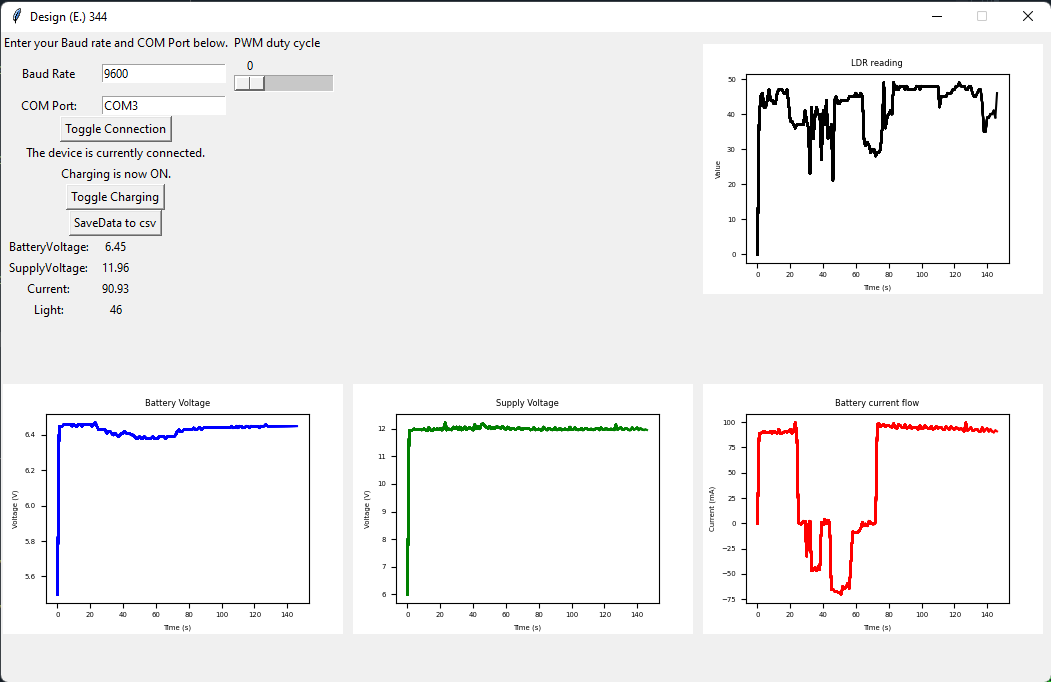
\includegraphics[width=1\linewidth]{Figures/A9/GUI.png}
	\caption{Software GUI}
	\label{fig:GUI}
\end{figure}